\documentclass[border=8pt]{standalone}
\usepackage{mathpazo}
\usepackage{tikz}
\usetikzlibrary{arrows.meta,calc,decorations.pathreplacing}

\definecolor{stblue}{HTML}{7B97AD}
\definecolor{rwgold}{HTML}{B8995E}
\definecolor{sage}{HTML}{7A9A7E}
\definecolor{terracotta}{HTML}{C47A6A}
\definecolor{dkbrown}{HTML}{3D3530}
\definecolor{wmgray}{HTML}{7B7067}
\definecolor{goldfill}{HTML}{F5EFE4}
\definecolor{bluefill}{HTML}{E8EDF2}

\begin{document}
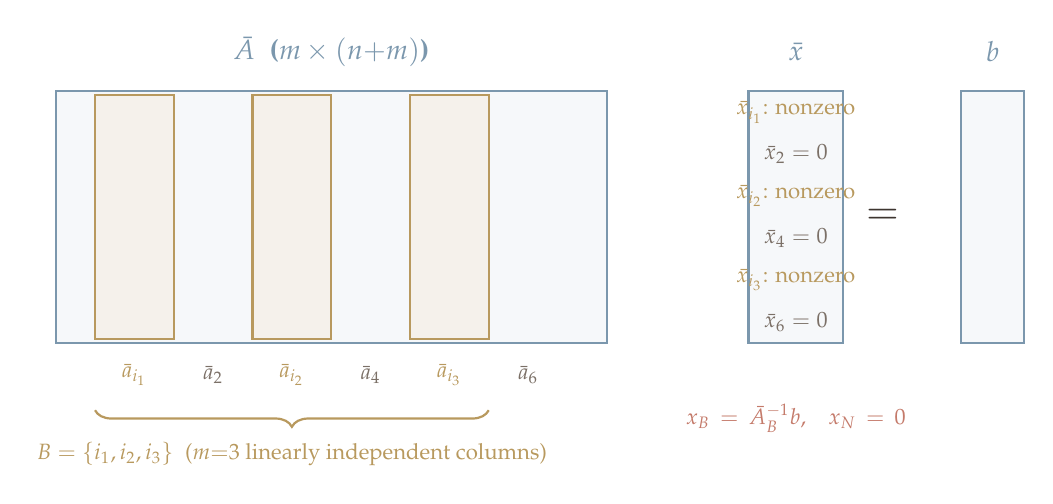
\begin{tikzpicture}[font=\small]

% === Augmented matrix A-bar ===
% Big rectangle for A-bar: 7 columns x 3 rows
\def\matW{7.0}
\def\matH{3.2}
\def\colW{1.0}

% Background rect
\fill[bluefill,opacity=0.4] (0,0) rectangle (\matW,\matH);
\draw[stblue,thick] (0,0) rectangle (\matW,\matH);

% Basis columns highlighted (columns i1, i2, i3 ~ positions 1, 3, 5)
\fill[goldfill,opacity=0.7] (0.5,0.05) rectangle (1.5,\matH-0.05);
\draw[rwgold,thick] (0.5,0.05) rectangle (1.5,\matH-0.05);

\fill[goldfill,opacity=0.7] (2.5,0.05) rectangle (3.5,\matH-0.05);
\draw[rwgold,thick] (2.5,0.05) rectangle (3.5,\matH-0.05);

\fill[goldfill,opacity=0.7] (4.5,0.05) rectangle (5.5,\matH-0.05);
\draw[rwgold,thick] (4.5,0.05) rectangle (5.5,\matH-0.05);

% Column labels below
\node[rwgold,font=\footnotesize\bfseries] at (1.0,-0.4) {$\bar{a}_{i_1}$};
\node[wmgray,font=\footnotesize] at (2.0,-0.4) {$\bar{a}_2$};
\node[rwgold,font=\footnotesize\bfseries] at (3.0,-0.4) {$\bar{a}_{i_2}$};
\node[wmgray,font=\footnotesize] at (4.0,-0.4) {$\bar{a}_4$};
\node[rwgold,font=\footnotesize\bfseries] at (5.0,-0.4) {$\bar{a}_{i_3}$};
\node[wmgray,font=\footnotesize] at (6.0,-0.4) {$\bar{a}_6$};

% Matrix label
\node[stblue,font=\normalsize\bfseries] at (3.5,\matH+0.5) {$\bar{A}$\; ($m \times (n{+}m)$)};

% === x-bar vector ===
\def\xOff{8.8}
\def\xW{1.2}
\fill[bluefill,opacity=0.4] (\xOff,0) rectangle (\xOff+\xW,\matH);
\draw[stblue,thick] (\xOff,0) rectangle (\xOff+\xW,\matH);

% Entries of x-bar (6 entries from top to bottom)
\def\rowH{0.533}
\node[rwgold,font=\footnotesize] at (\xOff+0.6, \matH - 0.5*\rowH) {$\bar{x}_{i_1}$: nonzero};
\node[wmgray,font=\footnotesize] at (\xOff+0.6, \matH - 1.5*\rowH) {$\bar{x}_2 = 0$};
\node[rwgold,font=\footnotesize] at (\xOff+0.6, \matH - 2.5*\rowH) {$\bar{x}_{i_2}$: nonzero};
\node[wmgray,font=\footnotesize] at (\xOff+0.6, \matH - 3.5*\rowH) {$\bar{x}_4 = 0$};
\node[rwgold,font=\footnotesize] at (\xOff+0.6, \matH - 4.5*\rowH) {$\bar{x}_{i_3}$: nonzero};
\node[wmgray,font=\footnotesize] at (\xOff+0.6, \matH - 5.5*\rowH) {$\bar{x}_6 = 0$};

% Label
\node[stblue,font=\normalsize\bfseries] at (\xOff+0.6,\matH+0.5) {$\bar{x}$};

% === equals sign ===
\node[dkbrown,font=\Large] at (\xOff+\xW+0.5, \matH/2) {$=$};

% === b vector ===
\def\bOff{11.5}
\fill[bluefill,opacity=0.4] (\bOff,0) rectangle (\bOff+0.8,\matH);
\draw[stblue,thick] (\bOff,0) rectangle (\bOff+0.8,\matH);
\node[stblue,font=\normalsize\bfseries] at (\bOff+0.4,\matH+0.5) {$b$};

% === Brace under basis columns ===
\draw[decorate,decoration={brace,amplitude=6pt,mirror},rwgold,thick]
  (0.5,-0.85) -- (5.5,-0.85)
  node[midway,below=8pt,rwgold,font=\footnotesize] {$B = \{i_1, i_2, i_3\}$ \;($m{=}3$ linearly independent columns)};

% === Annotation under x-bar ===
\node[terracotta,font=\footnotesize,text width=3.5cm,align=center] at (\xOff+0.6,-0.95)
  {$x_B = \bar{A}_B^{-1}b$,\quad $x_N = 0$};

\end{tikzpicture}
\end{document}
